% BDEC CreGen relation — paper-exact (ProSec2024 p.12, AND of two Sig.Verify,
% both under pk_U). Draws the PUBLIC-instance vs WITNESS boundary explicitly:
%   x = (c_{U,TA}, h_{U,TA}, ppk_{U,TA})   public
%   w = (pk_U, psk_{U,TA})                 witness (hidden)
% This is the figure for the public/witness separation question.
% Compile: pdflatex cregen_relation.tex
\documentclass[border=4pt]{standalone}
\usepackage{tikz}
\usepackage{newtxtext,newtxmath}
\usetikzlibrary{positioning,arrows.meta,fit,backgrounds,calc}
% Thesis macros used in labels (standalone figs don't inherit sakolab-thesis.sty):
\newcommand{\Sig}{\mathsf{Sig}}
\begin{document}
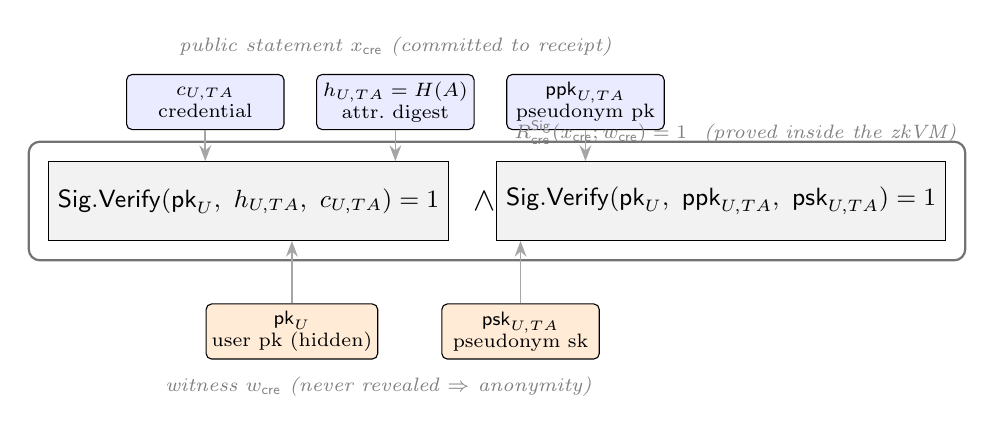
\begin{tikzpicture}[
  font=\small,>={Stealth[length=2mm]},
  pub/.style={draw,rounded corners=2pt,fill=blue!8,minimum width=20mm,minimum height=7mm,inner sep=2pt,align=center,font=\scriptsize},
  wit/.style={draw,rounded corners=2pt,fill=orange!16,minimum width=20mm,minimum height=7mm,inner sep=2pt,align=center,font=\scriptsize},
  ver/.style={draw,fill=gray!10,minimum width=44mm,minimum height=10mm,align=center},
  lbl/.style={font=\scriptsize\itshape,gray},
  flow/.style={->,semithick,gray!70},
]

% public inputs (top)
\node[pub] (c)   {$c_{U,TA}$\\\scriptsize credential};
\node[pub,right=4mm of c] (h)   {$h_{U,TA}=H(A)$\\\scriptsize attr.\ digest};
\node[pub,right=4mm of h] (ppk) {$\mathsf{ppk}_{U,TA}$\\\scriptsize pseudonym pk};
\node[lbl,above=1mm of h] {public statement $x_{\mathsf{cre}}$ (committed to receipt)};

% witnesses (bottom)
\node[wit,below=22mm of c,xshift=11mm]  (pku)  {$\mathsf{pk}_U$\\\scriptsize user pk (hidden)};
\node[wit,right=8mm of pku] (psk) {$\mathsf{psk}_{U,TA}$\\\scriptsize pseudonym sk};
\node[lbl,below=1mm of pku,xshift=11mm] {witness $w_{\mathsf{cre}}$ (never revealed $\Rightarrow$ anonymity)};

% the two verifications
\node[ver] (v1) at ($(c)!0.5!(pku)+(0,2mm)$) {$\mathsf{Sig.Verify}(\mathsf{pk}_U,\ h_{U,TA},\ c_{U,TA})=1$};
\node[ver,right=6mm of v1] (v2) {$\mathsf{Sig.Verify}(\mathsf{pk}_U,\ \mathsf{ppk}_{U,TA},\ \mathsf{psk}_{U,TA})=1$};
\node[font=\large] at ($(v1)!0.5!(v2)$) {$\wedge$};

% feed arrows
\draw[flow] (c)   -- (v1.north-|c);
\draw[flow] (h)   -- (v1.north-|h);
\draw[flow] (ppk) -- (v2.north-|ppk);
\draw[flow] (pku.north) -- (v1.south-|pku);
\draw[flow] (psk.north) -- (v2.south-|psk);

\begin{scope}[on background layer]
  \node[fit=(v1)(v2),draw=black!55,thick,rounded corners,inner sep=7pt] (zkbox){};
\end{scope}
% relation label placed ABOVE the box, clear of the witness arrows below
\node[lbl,above=1mm of zkbox.north east,anchor=east] {$R_{\mathsf{cre}}^{\Sig}(x_{\mathsf{cre}};w_{\mathsf{cre}})=1$\ \ (proved inside the zkVM)};
\end{tikzpicture}
\end{document}
